\documentclass[12pt]{article}
\usepackage[utf8]{inputenc}
\usepackage{float}
\usepackage{amsmath}


\usepackage[hmargin=3cm,vmargin=6.0cm]{geometry}
%\topmargin=0cm
\topmargin=-2cm
\addtolength{\textheight}{6.5cm}
\addtolength{\textwidth}{2.0cm}
%\setlength{\leftmargin}{-5cm}
\setlength{\oddsidemargin}{0.0cm}
\setlength{\evensidemargin}{0.0cm}

%misc libraries goes here
\usepackage{tikz}
\usetikzlibrary{automata,positioning}

\begin{document}

\section*{Student Information } 
%Write your full name and id number between the colon and newline
%Put one empty space character after colon and before newline
Full Name : Hakan Bostan \\
Id Number : 2098812 \\

% Write your answers below the section tags
\section*{Answer 1}

\subsection*{a.}
Strings in the form of $ x^iy^jz^k $ where $i,j,k\geq 0 $ and $ i=k$ or $i=j$
\subsection*{b.}
Strings in the form of $ w\$(x,y)^*w^R(x,y)^* $ where $w$ is a string composed of anynumber of "x"s and "y"s ($|w|>0$), while $(x,y)^*$ shows an arbitrarily long string composed of $x,y$s in any order.
\subsection*{c.}
$(x(xxxxxxxxx)^*)+((z,y)(z,y))^*$



\section*{Answer 2}

\subsection*{a.}
Assume that $L=\lbrace aa^R2^{|a|}: a\in {\lbrace 1,2 \rbrace }^* \rbrace $ is context free. \\
Let $p$ be the number from the pumping lemma, also let $|a|=p$ and $s=aa^R2^p$ therefore $|s| = 3p$\\
$s=uvwxy$ and $|vwx|\leq p , |vx|>0 $\\
There are 5 ways to choose the piece of string $vwx$ and assume we pump v and x up(e.g. $s=uv^2wx^2y$):\\
\textbf{Case 1:} all $v,w,x$ is in $a$ $\rightarrow |a^{R'}| \neq p $\\
\textbf{Case 2:} all $v,w,x$ is in $a^R$ $\rightarrow |a^{R'}| \neq |a|  $\\
\textbf{Case 3:} all $v,w,x$ is in $2^p$ $\rightarrow |2^p| \neq |a'| $\\
\textbf{Case 4:}\\
\indent \textbf{•} $v$ in $a$ , $x$ in $a^R$ , $w$ in $a$ or $a^R $ $\rightarrow |2^p| \neq |a'| $\\
\indent \textbf{•} $v$ in $a$ and $a^R$ , $x$ in $a^R$ , $w$ in $a^R $ $\rightarrow |2^p| \neq |a'| $\\
\indent \textbf{•} $v$ in $a$ , $x$ in $a$ and $a^R$ , $w$ in $a  $ $\rightarrow |2^p| \neq |a'| $\\
\textbf{Case 5:}\\
\indent \textbf{•} $v$ in $a^R$ , $x$ in $2^p$, $w$ in $a^r $ or $2^p$ $\rightarrow |a| \neq |a^{R'}| $\\
\indent \textbf{•} $v$ in $a^R$ and $2^p$ , $x$ in $2^p$, $w$ in $2^p$ $\rightarrow |2^{p'}| \neq |a| $\\
\indent \textbf{•} $v$ in $a^R$ , $x$ in $a^R$ and $2^p$, $w$ in $a^R$ $\rightarrow |2^{p'}| \neq |a| $\\
Since all of these cases fail, we can safely conclude that $L$ is not a CFL.
\subsection*{b.}
We can create a PDA for A. If we push a symbol to the stack for every character we read until the end of "y"s, and then while taking "z"s as input, for each "z" we pop a symbol from the stack, if stack becomes empty before end of input or if input ends before stack becomes empty we reject the string. If input ends just as the stack becomes empty we accept the string. Since we can create a PDA, we can say that A is a CFL.\\
\\
$B=\lbrace x^ny^m : n,m\geq 0 \rbrace \cap \lbrace w : |w|\leq 200$ and $w\in \sum^* \rbrace = \lbrace x^ny^m: 0\leq n,m \leq 100$. Since both strings that intersect in this equation are regular (We can create a DFA for each one). From the closure properties of Regular Languages we can say that B is also a regular language.\\
\\
Since A is a CFL and B is a Regular language, from the closure properties of CFLs, we can say that $A\setminus B =  A\cap \overline{B}$ is a CFL.(From the theorem that states intersection of context-free languages and regular languages are context-free)
\subsection*{c.}
Assume that $L=\lbrace a^nb^mz^{n*m}: n,m\geq 0 \rbrace $ is context free. \\
Let $p$ be the number from the pumping lemma, $s=a^p b^p c^{pp}$ therefore $|s| = 2p+p^2$\\
$s=uvwxy$ and $|vwx|\leq p , |vx|>0 $\\
There are 5 ways to choose the piece of string $vwx$ and assume we pump v and x up(e.g. $s=uv^2wx^2y$):\\
\textbf{Case 1:} all $v,w,x$ is in $a^n$ $\rightarrow {n*m} \neq n'*m $\\
\textbf{Case 2:} all $v,w,x$ is in $b^m$ $\rightarrow {n*m} \neq n*m' $\\
\textbf{Case 3:} all $v,w,x$ is in $c^{n*m}$ $\rightarrow {n*m} \neq (n*m)' $\\
\textbf{Case 4:}\\
\indent \textbf{•} $v$ in $a^n$ , $x$ in $n^b$ , $w$ in $a^n$ or $b^m$ $\rightarrow n'*m' \neq n*m $\\
\indent \textbf{•} $v$ in $a^n$ and $b^m$ , $x$ in $b^m$ , $w$ in $b^m $ $\rightarrow n'*m' \neq n*m $\\
\indent \textbf{•} $v$ in $a^n$ , $x$ in $a^n$ and $b^m$ , $w$ in $a^n  $ $\rightarrow n'*m' \neq n*m $\\
\textbf{Case 5:}\\
\indent \textbf{•} $v$ in $b^m$ , $x$ in $c^{n*m}$, $w$ in $b^m $ or $c^{n*m}$ $\rightarrow n*m' \neq (n*m)' $\\
\indent \textbf{•} $v$ in $b^m$ and $c^{n*m}$ , $x$ in $c^{n*m}$, $w$ in $c^{n*m}$ $\rightarrow n*m' \neq (n*m)' $\\
\indent \textbf{•} $v$ in $b^m$ , $x$ in $b^m$ and $c^{n*m}$, $w$ in $c^{n*m}$ $\rightarrow n*m' \neq (n*m) $\\
Since all of these fail, we can safely conclude that $L$ is not a CFL.
\subsection*{d.}
L is a CFL with grammar G:\\
S $\rightarrow$ 1A22\\
A $\rightarrow$ 1A2 $|$ $ \epsilon$\\
So $\overline{L}$ needs further investigation.\\
$\overline{L} = \sum^* - L = L_a \cup L_b \cup L_c \cup L_d$ where \\
$L_a= \lbrace 1^n 2^m : m < n \rbrace$\\
$L_b= \lbrace 1^n 2^m : 2n<m \rbrace$\\
$L_c= \lbrace 2(1,2)^* \rbrace $\\
$L_d= \lbrace 1(1^*) 2(2^*)1(1,2)^* \rbrace $

$L_a$ has the grammar F:\\
S $\rightarrow$ 1S2 $|$ A\\
A $\rightarrow$ 1B\\
B $\rightarrow$ 1B $|$ $\lambda$\\

$L_b$ has the grammar H:\\
S $\rightarrow$ 1S22 $|$ A\\
A $\rightarrow$ B2\\
B $\rightarrow$ B2 $|$ $\lambda$\\

$L_c$ and $L_d$ are regular languages because we can express them with above regular expressions. Since they are regular, they are contex-free at the same time.\\
So $\overline{L}$ is just the union of 4 context-free languages. Since context-free languages are closed under union we can safely say that $L_4 = \overline{L}$ is a context-free language. Here is the grammar for $L_4$:\\
S $\rightarrow$ $S_1$ $|$ $S_2$ $|$ $S_3$ $|$ $S_4$ \\
$S_1$ $\rightarrow$ 1$S_1$2 $|$ A\\
A $\rightarrow$ 1B\\
B $\rightarrow$ 1B $|$ $\lambda$\\
$S_2$ $\rightarrow$ 1$S_2$22 $|$ X\\
X $\rightarrow$ Y2\\
Y $\rightarrow$ Y2 $|$ $\lambda$\\
$S_3$ $\rightarrow$ 2K\\
K $\rightarrow$ 1K $|$ 2K $|$ $\lambda$\\
$S_4$ $\rightarrow$ 1L2M1K\\
L $\rightarrow$ 1L $|$ $\lambda$\\
M $\rightarrow$ 2M $|$ $\lambda$\\








\section*{Answer 3}


\subsection*{a.}
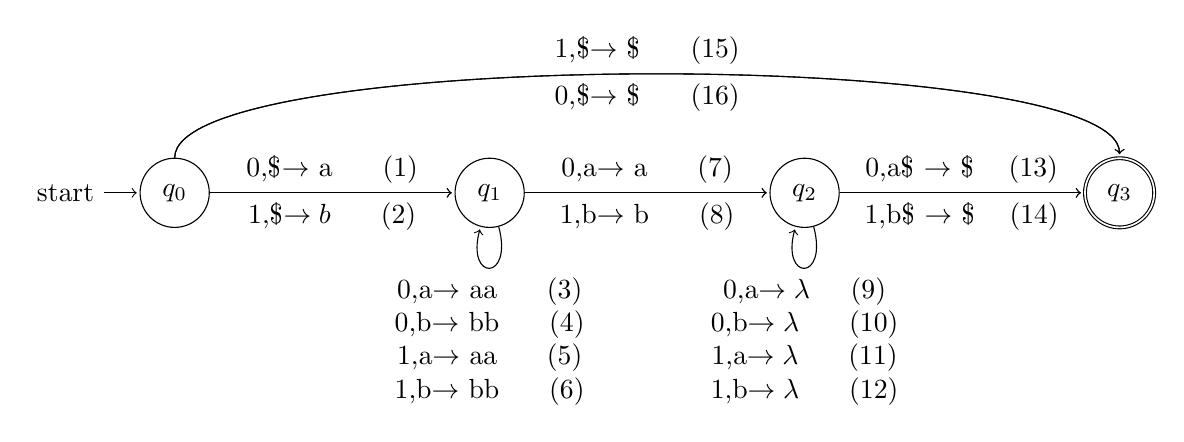
\begin{tikzpicture}[shorten >=1pt,node distance=4cm,on grid,auto]
	\node[state,initial] (q_0) {$q_0$};
	\node[state] (q_1) [right=of q_0] {$q_1$};
	\node[state] (q_2) [right=of q_1] {$q_2$};
	\node[state,accepting](q_3) [right=of q_2] {$q_3$};
		\path[->]
		(q_0) edge node [swap]{1,\$$ \rightarrow b$ \hspace{4mm} (2)} (q_1)
			  edge node  {0,\$$ \rightarrow$ a \hspace{4mm} (1)} (q_1)
			  edge [out=90,in=90,looseness=0.3] node {1,\$$ \rightarrow $ \$ \hspace{4mm} (15)} (q_3)
			  edge [out=90,in=90,looseness=0.3] node [swap] {0,\$$ \rightarrow $ \$ \hspace{4mm} (16)} (q_3)
		(q_1) edge [loop below]node [ align=center]{0,a$ \rightarrow$ aa \hspace{4mm} (3) \\ 0,b$ \rightarrow$ bb \hspace{4mm} (4) \\ 1,a$ \rightarrow$ aa \hspace{4mm} (5)\\ 1,b$ \rightarrow$ bb \hspace{4mm} (6)} (q_1)
		(q_1) edge node {0,a$ \rightarrow$ a \hspace{4mm} (7)} (q_2)
			  edge node [swap] {1,b$ \rightarrow$ b \hspace{4mm} (8)} (q_2)
		(q_2) edge [loop below]node [ align=center]{0,a$ \rightarrow \lambda $\hspace{4mm} (9) \\ 0,b$ \rightarrow \lambda $ \hspace{4mm} (10) \\ 1,a$ \rightarrow \lambda $ \hspace{4mm} (11)\\ 1,b$ \rightarrow \lambda $ \hspace{4mm} (12)} (q_2)
		(q_2) edge node {0,a\$ $ \rightarrow $ \$ \hspace{2mm} (13)} (q_3)
			  edge node [swap] {1,b\$ $ \rightarrow$ \$  \hspace{2mm} (14)} (q_3);
\end{tikzpicture}
\subsection*{b.}
State:$q_0$	\hspace{4mm} Input: -	\hspace{4.5mm} 	Transition:-		\hspace{6.5mm} New State:-			\hspace{6mm} Stack:\$ \\
State:$q_0$	\hspace{4mm} Input: 0	\hspace{4mm} 	Transition: 1		\hspace{4mm} New State:$q_1$		\hspace{4mm} Stack:\$a \\
State:$q_1$	\hspace{4mm} Input: 1	\hspace{4mm} 	Transition:	5   	\hspace{4mm} New State:$q_1$		\hspace{4mm} Stack:\$aa \\
State:$q_1$	\hspace{4mm} Input: 0	\hspace{4mm} 	Transition:	7 		\hspace{4mm} New State:$q_2$		\hspace{4mm} Stack:\$aa \\
State:$q_2$	\hspace{4mm} Input: 0	\hspace{4mm} 	Transition:	9 		\hspace{4mm} New State:$q_2$		\hspace{4mm} Stack:\$a \\
State:$q_2$	\hspace{4mm} Input: 0	\hspace{4mm}  	Transition:	13 		\hspace{2mm} New State:$q_3$		\hspace{4mm} Stack:\$ \tikz\fill[scale=0.4](0,.35) -- (.25,0) -- (1,.7) -- (.25,.15) -- cycle;
\subsection*{c.}

State:$q_0$	\hspace{4mm} Input: -	\hspace{4.5mm} 	Transition:-		\hspace{6.5mm} New State:-			\hspace{6mm} Stack:\$ \\
State:$q_0$	\hspace{4mm} Input: 0	\hspace{4mm} 	Transition: 1		\hspace{4mm} New State:$q_1$		\hspace{4mm} Stack:\$a \\
State:$q_1$	\hspace{4mm} Input: 0	\hspace{4mm} 	Transition:	3   	\hspace{4mm} New State:$q_1$		\hspace{4mm} Stack:\$aa \\
State:$q_1$	\hspace{4mm} Input: 1	\hspace{4mm} 	Transition: 5 		\hspace{4mm} New State:$q_1$		\hspace{4mm} Stack:\$aaa \\
State:$q_1$	\hspace{4mm} Input: 0	\hspace{4mm} 	Transition:	7 		\hspace{4mm} New State:$q_2$		\hspace{4mm} Stack:\$aaa \\
State:$q_2$	\hspace{4mm} Input: 0	\hspace{4mm}  	Transition:	9 		\hspace{2mm} New State:$q_2$		\hspace{4mm} Stack:\$aa \tikz [x=1.4ex,y=1.4ex,line width=.2ex, red] \draw (0,0) -- (1,1) (0,1) -- (1,0);\\
Ended up in a non-accepting state.\\
\vspace{5mm}
\\State:$q_0$	\hspace{4mm} Input: -	\hspace{4.5mm} 	Transition:-		\hspace{6.5mm} New State:-			\hspace{6mm} Stack:\$ \\
State:$q_0$	\hspace{4mm} Input: 0	\hspace{4mm} 	Transition: 1		\hspace{4mm} New State:$q_1$		\hspace{4mm} Stack:\$a \\
State:$q_1$	\hspace{4mm} Input: 0	\hspace{4mm} 	Transition:	3   	\hspace{4mm} New State:$q_1$		\hspace{4mm} Stack:\$aa \\
State:$q_1$	\hspace{4mm} Input: 1	\hspace{4mm} 	Transition:	5 		\hspace{4mm} New State:$q_1$		\hspace{4mm} Stack:\$aaa \\
State:$q_1$	\hspace{4mm} Input: 0	\hspace{4mm} 	Transition:	3 		\hspace{4mm} New State:$q_1$		\hspace{4mm} Stack:\$aaaa \\
State:$q_1$	\hspace{4mm} Input: 0	\hspace{4mm}  	Transition:	7 		\hspace{2mm} New State:$q_2$		\hspace{4mm} Stack:\$aaa \tikz [x=1.4ex,y=1.4ex,line width=.2ex, red] \draw (0,0) -- (1,1) (0,1) -- (1,0);\\
Ended up in a non-accepting state.\\
\vspace{5mm}
\\State:$q_0$	\hspace{4mm} Input: -	\hspace{4.5mm} 	Transition:-		\hspace{6.5mm} New State:-			\hspace{6mm} Stack:\$ \\
State:$q_0$	\hspace{4mm} Input: 0	\hspace{4mm} 	Transition: 1		\hspace{4mm} New State:$q_1$		\hspace{4mm} Stack:\$a \\
State:$q_1$	\hspace{4mm} Input: 0	\hspace{4mm} 	Transition:	3   	\hspace{4mm} New State:$q_1$		\hspace{4mm} Stack:\$aa \\
State:$q_1$	\hspace{4mm} Input: 1	\hspace{4mm} 	Transition:	5 		\hspace{4mm} New State:$q_1$		\hspace{4mm} Stack:\$aaa \\
State:$q_1$	\hspace{4mm} Input: 0	\hspace{4mm} 	Transition:	3 		\hspace{4mm} New State:$q_1$		\hspace{4mm} Stack:\$aaaa \\
State:$q_1$	\hspace{4mm} Input: 0	\hspace{4mm}  	Transition:	3 		\hspace{2mm} New State:$q_1$		\hspace{4mm} Stack:\$aaaaa \tikz [x=1.4ex,y=1.4ex,line width=.2ex, red] \draw (0,0) -- (1,1) (0,1) -- (1,0);\\
Ended up in a non-accepting state.\\
\vspace{5mm}
\\State:$q_0$	\hspace{4mm} Input: -	\hspace{4.5mm} 	Transition:-		\hspace{6.5mm} New State:-			\hspace{6mm} Stack:\$ \\
State:$q_0$	\hspace{4mm} Input: 0	\hspace{4mm} 	Transition: 1		\hspace{4mm} New State:$q_1$		\hspace{4mm} Stack:\$a \\
State:$q_1$	\hspace{4mm} Input: 0	\hspace{4mm} 	Transition:	7   	\hspace{4mm} New State:$q_2$		\hspace{4mm} Stack:\$a \\
State:$q_2$	\hspace{4mm} Input: 1	\hspace{4mm} 	Transition: 11 		\hspace{4mm} New State:$q_2$		\hspace{4mm} Stack:\$ \tikz [x=1.4ex,y=1.4ex,line width=.2ex, red] \draw (0,0) -- (1,1) (0,1) -- (1,0);\\
Input not exhausted and stuck in a non-accepting state.\\


\section*{Answer 4}

\subsection*{a.}
Since $R$ is regular $\overline{R}$ is also regular, by the closure properties of regular languages. We can also show $L_2\setminus R$ as $L_2 \cap \overline{R}$. Intersection of a CFL with a regular language is also a CFL by closure properties, so  $L_2 \cap \overline{R}$ is context-free. $L_1 \cup (L_2 \cap \overline{R})$ is union of two context-free languages, again by the closure properties of context free languages, $L_1 \cup (L_2 \cap \overline{R})$ is also a context-free language. And since $L_1 \cup (L_2 \setminus R ) = L_1 \cup (L_2 \cap \overline{R})$, we can conclude that $L_1 \cup (L_2 \setminus R )$ is a context-free language.
\\
\\
$L_1 \cup L_2$ is a context-free language. So lets call $L_1 \cup L_2$, $L_3$. So we need to determine if $R\setminus L_3$ is CFL or not. $ R\setminus L_3 $ $=$ $ R \cap \overline{L_3}$. $L_3$ is CFL and CFL's are not closed under complementation. So we cannot say whether if $ \overline{L_3} $ is a CLF or not. So if $\overline{L_3}$ is CFL, then it follows that $R \cap \overline{L_3}$ is CFL.
\subsection*{b.}
\begin{tikzpicture}[shorten >=1pt,node distance=2cm,on grid,auto]
	\node (1) {$S$};
	\node (2) [below left=of 1] {$X$};
	\node (3) [below right=of 1] {$Y$};
	\node (4) [below left =of 2] {$X$};
	\node (5) [below right=of 2] {$x$};
	\node (6) [below =of 3] {$y$};
	\node (7) [below =of 4] {$x$};
	\path
		(1) edge node {}(2)
		(1) edge node {}(3)
		(2) edge node {}(4)
		(2) edge node {}(5)
		(3) edge node {}(6)
		(4) edge node {}(7);
		
\end{tikzpicture}

\begin{tikzpicture}[shorten >=1pt,node distance=2cm,on grid,auto]
	\node (1) {$S$};
	\node (2) [below left= of 1]{$xx$};
	\node (4) [below right=of 1]{$Y$};
	\node (5) [below =of 4]{$y$};
	\path
		(1) edge node {} (2)
		(1) edge node {} (4)
		(4) edge node {} (5);
		
\end{tikzpicture}

Since both of the above trees yield the string $xxy$, we can cleary say that there is an ambiguity in the grammar G.
\subsection*{c.}
$a^nb^nc^n$ is a language that can be accepted by M but not by N. M achieves this by every time it takes an input character $a$, it pushes a symbol to both of the stacks. So when "a"s end there are two stacks which have exactly as many symbols as number of "a"s. Then when taking "b"s as input it pops a symbol from the first stack, if stack becomes empty and there are still "b"s or if "b"s end but there are still symbols in the first stack, it rejects the string. We do the same thing with "c"s but with the second stack. If we end up with both stacks empty and no more input, we accpet the string. But since N doesn't have the second stack, there is no way to check the number of "c"s against number of "a"s or "b"s. Therefore M is more "powerful" than N because it can $remember$ more things than M(i.e. both the number of "a"s and "b"s in the example).




\end{document}

​

